\subsection{BuyingController}
I BuyingController klassen er der et par metoder i spil. Vi har en boolean "isALLFieldsInSeriesOwned". Den tjekker om begge grunde af samme farve er ejet, når spilleren lander på et af de to felter. For at dette kan lade sig gøre, så tjekker den spillerens position (den grund, som spilleren står på) og felterne ved siden af, samt den farve de har. Der efter kigger den på om spilleren ejer begge felter (da det fordobler huslejen for feltet, når en modspiller lander på feltet). Hvis spilleren ikke ejer begge felter (fordi det andet felt er solgt eller ikke ejes endnu), så bliver vores boolean falsk, og resulterer dermed ikke i fordoblet husleje. Dette kan ses på billedet nedenfor:

\begin{figure}[H]
    \centering
    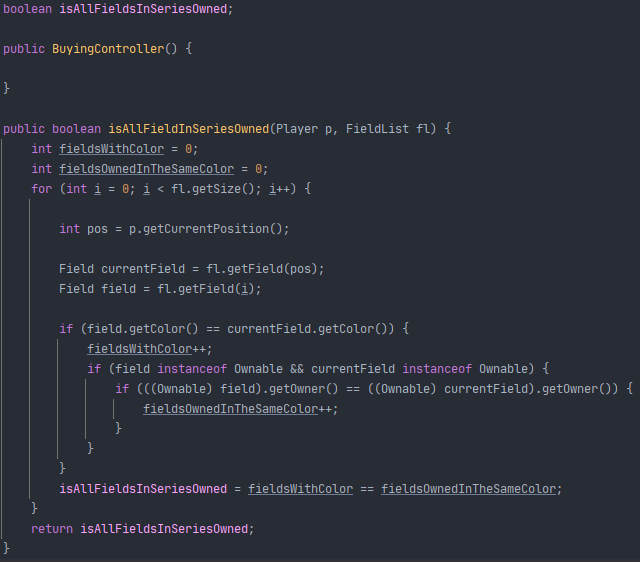
\includegraphics[width=0.7\textwidth]{sources/7_implementering/BuyingController.PNG}
    \caption{Metode der tjekker, om spilleren ejer begge felter af samme farve}
    \label{fig:chance}
\end{figure}

Den næste metode er "buyNextPossibleField". Her tjekker metoden for det næste mulige felt, som ikke er ejet af nogle spillere. Når det felt er fundet, så rykkes spilleren over til det felt, og køber det. Den rykker selvfølgelig spilleren i den rigtige retning rundt på spillepladen. Det er gjort ved en forkommando, som tager udganspunkt i spillerens nuværende position, og derefter tjekker de næste felter, for at se om de kan købes (ownable). Dette kan ses på billedet nedenfor
\begin{figure}[H]
    \centering
    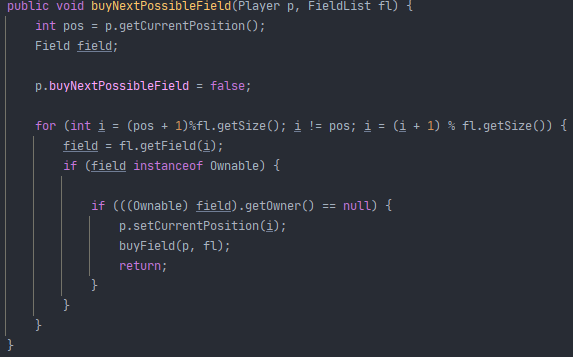
\includegraphics[width=0.7\textwidth]{sources/7_implementering/BuyingControllerMethod2.PNG}
    \caption{Rykker spilleren til det næste mulige felt, og køber der}
    \label{fig:chance}
\end{figure}

Den sidste metode er "buyField". Denne metode gør det muligt for spilleren at købe et ledigt felt. Det gøres ud fra spillerens position, hvor metoden tjekker om det er et felt der kan købes. Hvis feltet kan købes, så går metoden ind i "player" klassen og hæver det beløb, som er tilknyttet feltet. Hvis feltet allerede er solgt til en anden spiller, så tager metoden fat i metoden "isAllFieldInSeriesOwned", for at som om spilleren har været så uheldig, at spilleren skal betale den dobbelte husleje. Hvis der ikke er dobbelt husleje, så betaler spilleren den normale pris til ejeren af feltet. Dette kan ses på billedet nedenfor:
\begin{figure}[H]
    \centering
    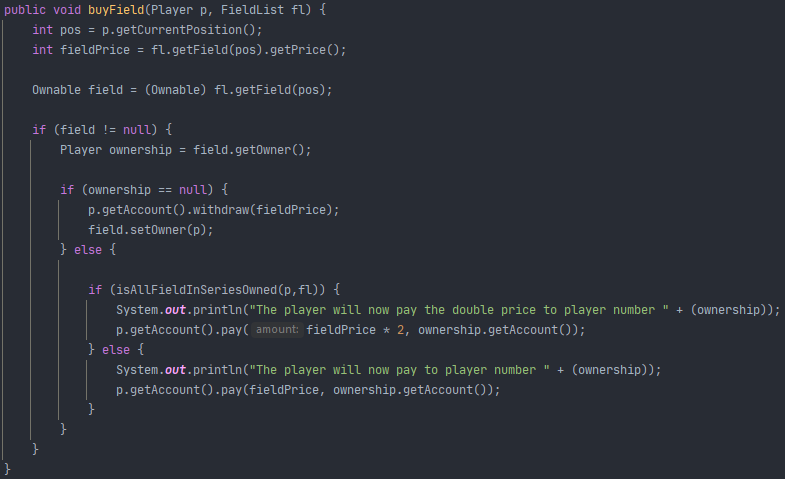
\includegraphics[width=0.7\textwidth]{sources/7_implementering/buyField.PNG}
    \caption{Metode for at sælge felter og tjekke husleje}
    \label{fig:chance}
\end{figure}
